%% Beginning of file 'SN2020jgb.tex'
%% using aastex version 6.3
\documentclass[twocolumn]{aastex631}

\newcommand\sn{SN\,2020jgb}
\newcommand\trpeak{$t_{r,\mathrm{peak}}$}
\newcommand\tfl{$t_\mathrm{fl}$}

\shorttitle{\sn}
\shortauthors{Authors et al.}
\graphicspath{{./}{figures/}}

\begin{document}

\title{\sn}

\author{Authors}
\affiliation{Center for Interdisciplinary Exploration and Research in Astrophysics (CIERA), Department of Physics and Astronomy, Northwestern University, 2145 Sheridan Road, Evanston, IL 60208, USA}

\begin{abstract}

\end{abstract}

\keywords{keywords}

\section{Introduction} \label{sec:intro}
\section{Observations} \label{sec:obs}
\subsection{Detection and Classification}
\sn\ was first discovered by the Zwicky Transient Facility \citep[ZTF;][]{ZTF2019a,ZTF2019b} on 2020 May 03.463 UT (MJD 58972.463) with the 48-inch Samuel Oschin Telescope (P48) at Palomar Observatory. The internal designation is ZTF20aayhacx. It was detected at a magnitude of 19.86 in ZTF $g$-band, and J2000 coordinates $\alpha=17^\mathrm{h}53^\mathrm{m}12^\mathrm{s}.651$, $\delta=-00^\circ51'21''.81$. The last non-detection was on 2020 April 27.477 (MJD 58966.477; 5.99 days before the first detection) up to a limiting magnitude of 20.7 in ZTF $r$-band.

\textbf{Classification, ...}

\subsection{Optical Photometry}
We obtained $gr$-band photometry of \sn\ with the ZTF camera. A Galactic extinction of $E(B-V)=0.404$ is reported by the maps of \citet{Schlafly2011}, for which we correct all our photometry using the extinction model proposed by \citet{Fitzpatrick1999}. We do not account for any additional host extinction due to the lack of any \ion{Na}{1} D absorption in our spectra (\textbf{Is it in the outskirt?}).
\begin{figure*}
    \centering
    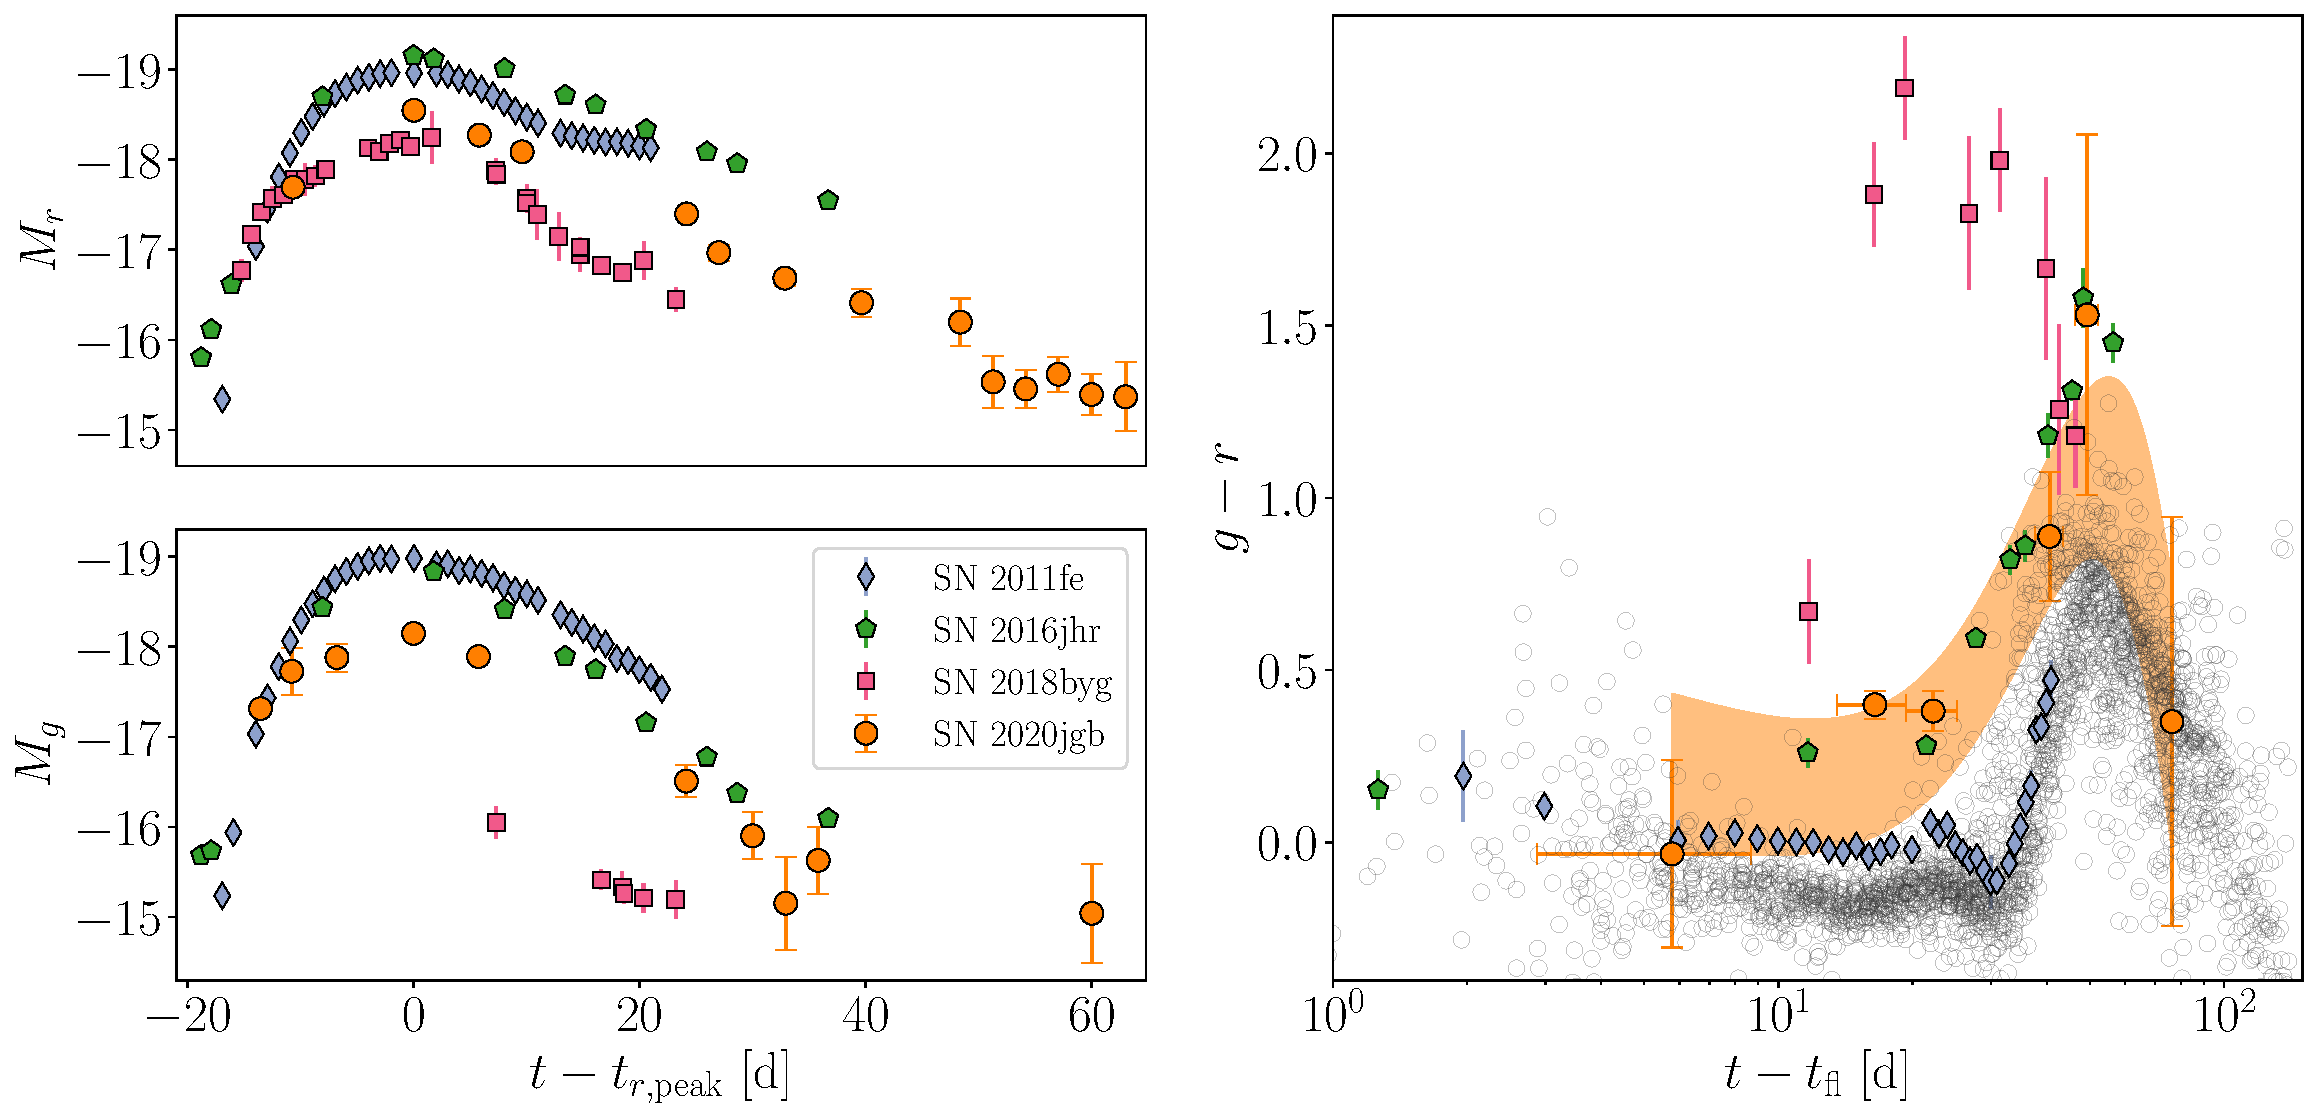
\includegraphics[width=\textwidth]{photometry.pdf}
    \label{fig:photometry}
    \caption{\textit{Left}: comparison of the multi-color ($g$ and $r$ bands) light curves of \sn\ to the normal SN Ia SN 2011fe and the He double detonation candidate SN 2018byg. \textit{Right}: comparison of $g-r$ color evolution to SN 2011fe and SN 2018byg, as well as 62 normal SNe Ia (open circles) with prompt observations within 5 days of first light by ZTF \citep{Bulla2020}. The shaded region denotes the 1-$\sigma$ credible interval of the color of SN 2020jgb until $\approx$40 days after the peak, estimated using Gaussian process.}
\end{figure*}

\subsection{Optical Spectroscopy}
\begin{deluxetable}{lrcccc}
\tabletypesize{\scriptsize}
\tablewidth{0pt}
\tablecaption{Spectroscopic Observations of \sn\label{tab:spectra}}
\tablehead{
\colhead{$t_\mathrm{obs}$} &
\colhead{Phase} &
\colhead{Telescope/} &
\colhead{$R$} &
\colhead{Range} &
\colhead{Air} \\
\colhead{(MJD)} &
\colhead{(d)} &
\colhead{Instrument} &
\colhead{$(\lambda/\Delta\lambda)$} &
\colhead{(\AA)} & 
\colhead{Mass}
}
\startdata
58,976.42 &  $-$9.7 & P60/SEDM & 100 & 3770--9220 & 1.23\\
58,982.12 & $-$4.2 & NOT/ALFOSC & 360 & 4000--9620 & 1.17\\
58,990.43 &  $+$3.9 & P60/SEDM & 100 & 3770--9220 &  1.23\\
58,997.44 & $+$10.7 & P60/SEDM & 100 & 3770--9220 &  1.29\\
58,998.41 & $+$11.6 & Shane/Kast & 1000? & 3620--10720 & 1.28\\
59,008.41 & $+$21.3 & P60/SEDM & 100 & 3770--9220 & 1.28\\
59,010.40 & $+$23.3 & P200/DBSP & 700 & 3200--9500 &  1.27\\
59,023.58 & $+$36.1 & Keck I/LRIS & 1100 & 3200--10250 & 2.04\\
59,107.29 & $+$117.3 & Keck I/LRIS & 1100 & 3200--10250 & 1.31\\
59,143.26 & $+$152.2 & Keck I/LRIS & 1100 & 3200--10250 & 2.16\\
\enddata
\tablecomments{Phase is measured relative to \trpeak\ in the host galaxy rest frame. The resolution $R$ is reported for the central region of the spectrum.}
\end{deluxetable}
\begin{figure}
    \centering
    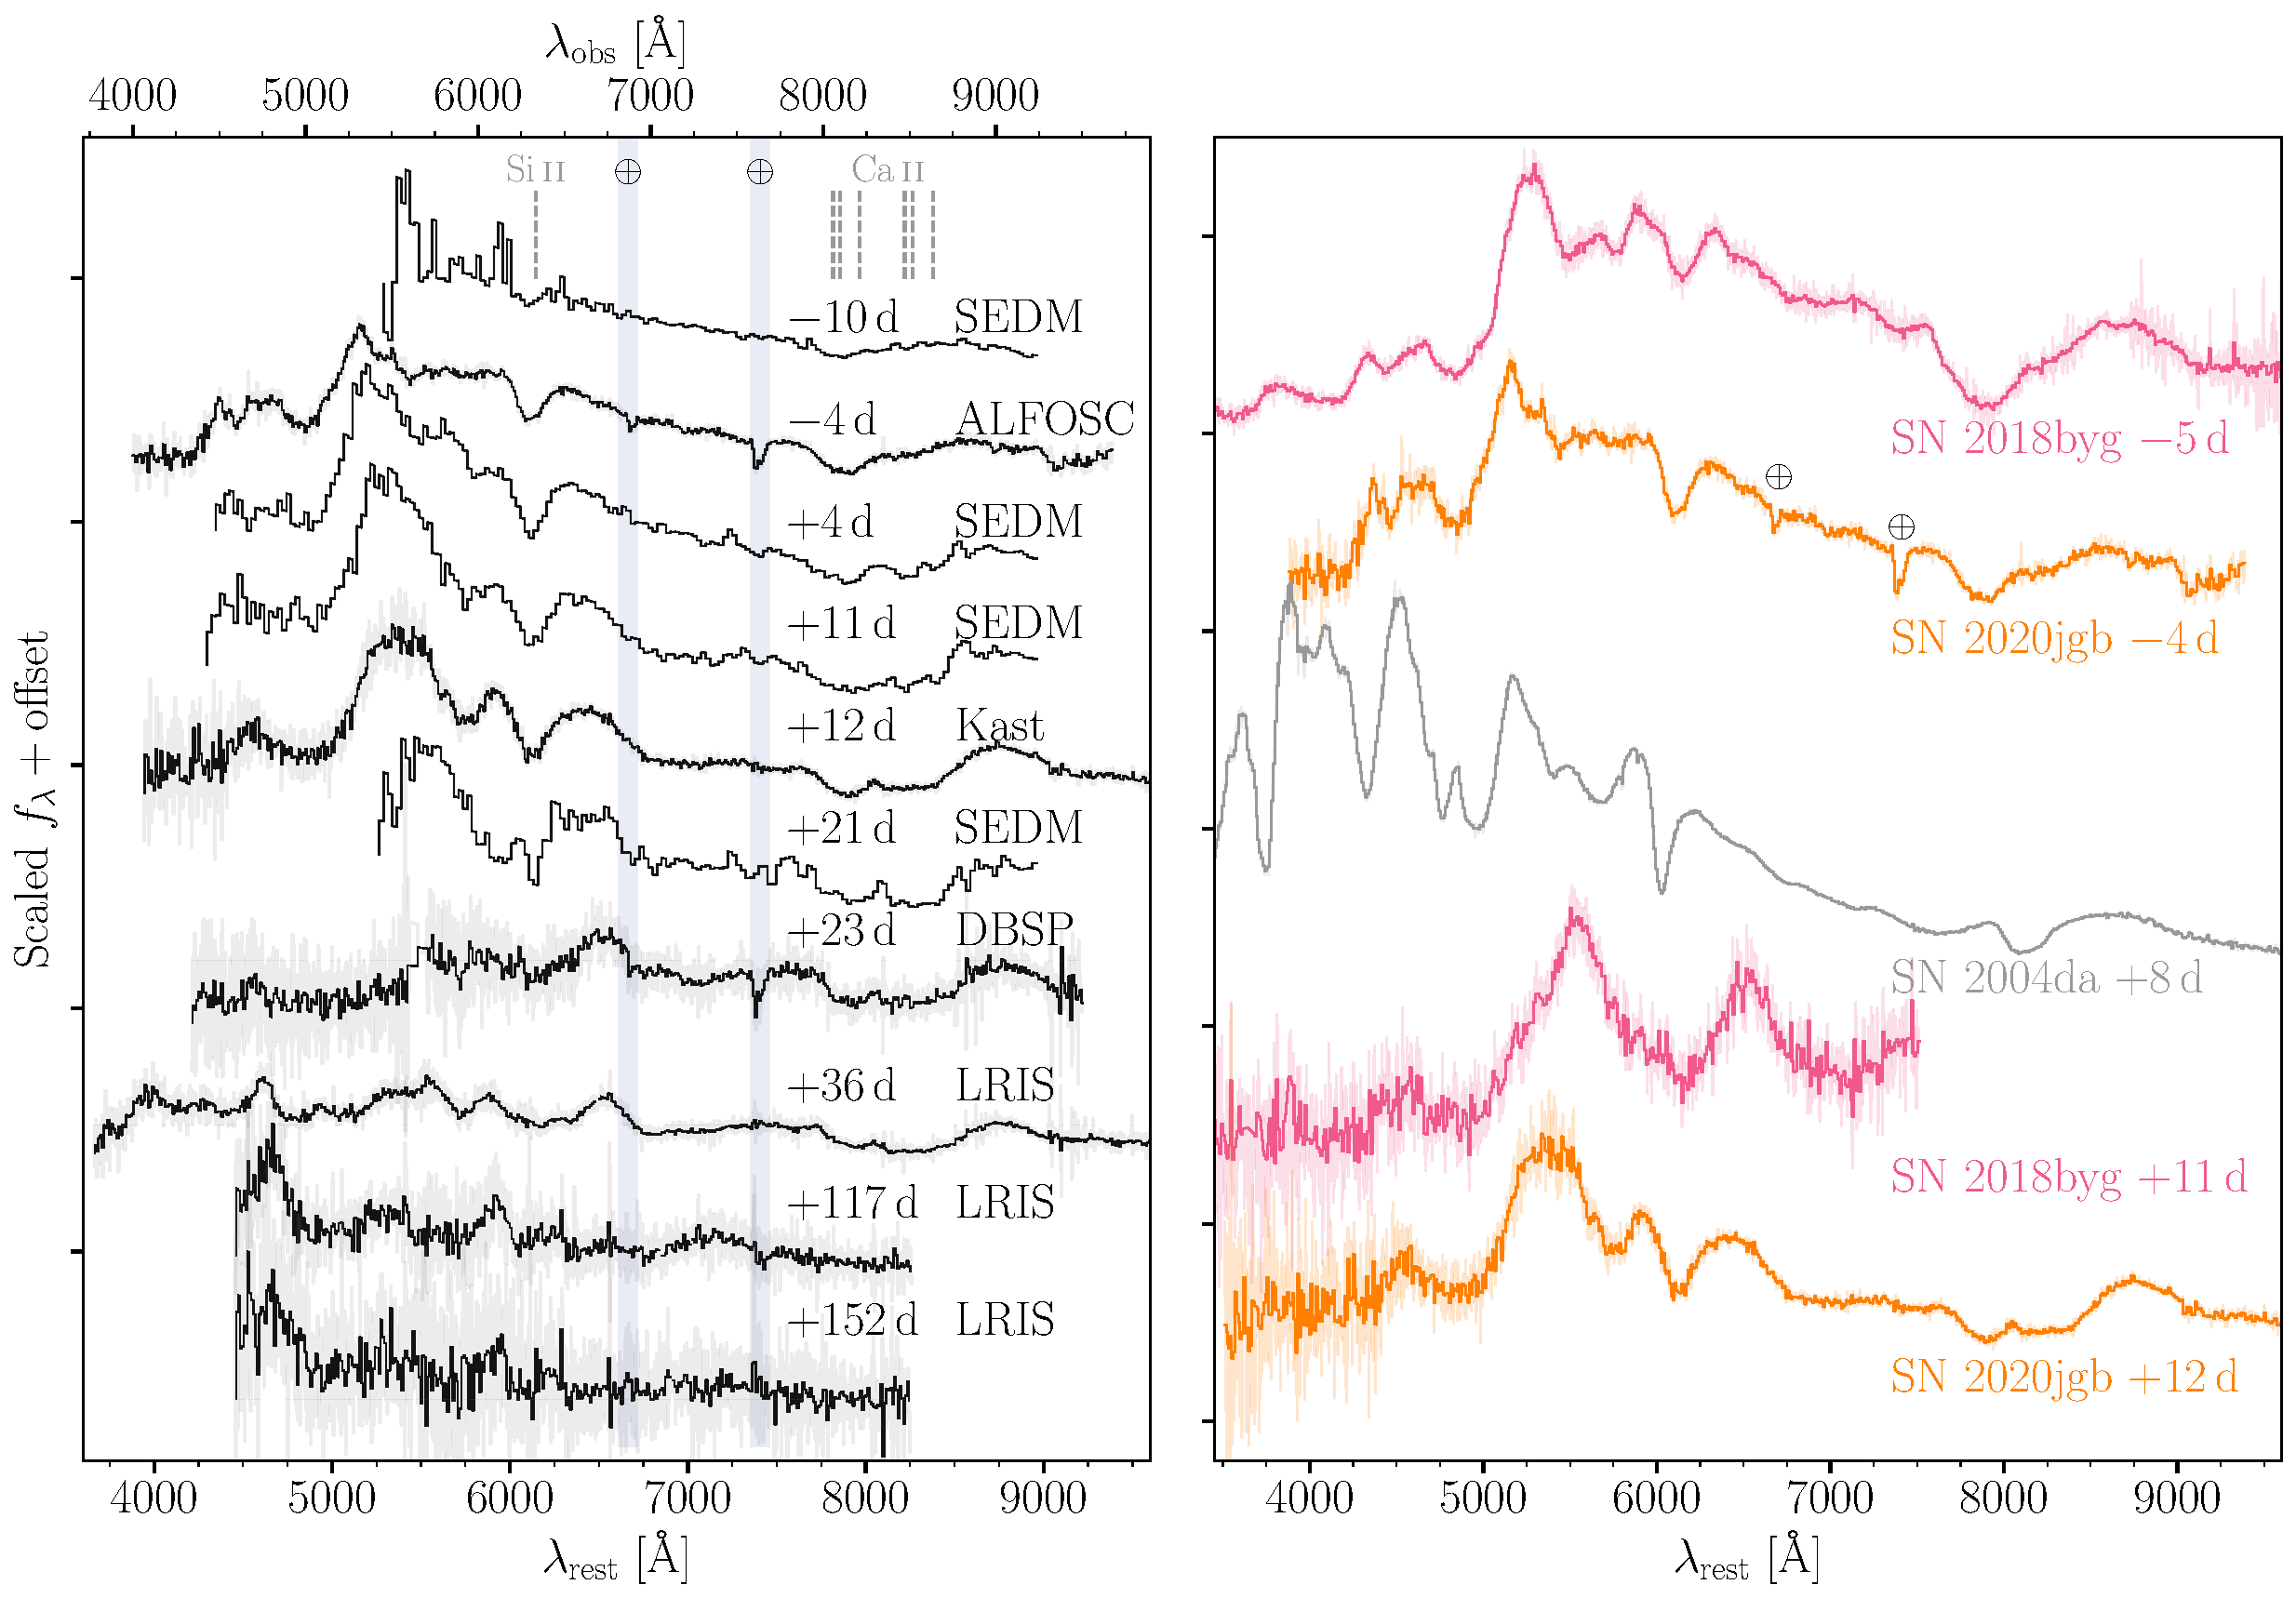
\includegraphics[width=\linewidth]{optical_spec_evolution.pdf}
    \label{fig:spec_evo}
    \caption{Optical spectroscopic sequence of \sn. Rest frame phases (days) relative to the $r$-band peak and instruments used are posted next to each spectrum. The black curves are binned spectra with a bin size of 10 \r{A}, except for the SEDm spectra, whose resolution is lower. The 1-$\sigma$ uncertainties of raw spectra are shown in grey. Only regions with SNR $>3$ after binning are plotted.} %The \ion{Si}{2} and \ion{Ca}{2} IRT absorption lines are indicated by the vertical dashed lines. The telluric lines are denoted by the earth symbol, ``$\earth$''.
\end{figure}

\subsection{Near-infrared (NIR) Spectroscopy}
We obtained one NIR spectrum of the transient using the Gemini near-infrared spectrometer \citep[GNIRS;][]{GNIRS1998} on the Gemini North telescope on 2020 June 9 ($\approx$22 days after $r$-band peak), for an integration time of 2400 s. The spectra were reduced with the \texttt{PypeIt} Python package \citep{pypeit:joss_pub,pypeit:zenodo}.

\section{Analysis} \label{sec:analysis}
\subsection{Photometric Properties}
\begin{itemize}
    \item sub-luminous
    \item first light time, peak time
    \item color evolution
\end{itemize}

\subsection{Spectroscopic Properties}
\begin{itemize}
    \item infrared \ion{Ca}{2} triplet (\ion{Ca}{2} IRT)
    \item tentative \ion{He}{1} absorption at $\approx$9900 \r{A}
\end{itemize}
\subsection{Optical Spectroscopy}
\begin{figure}
    \centering
    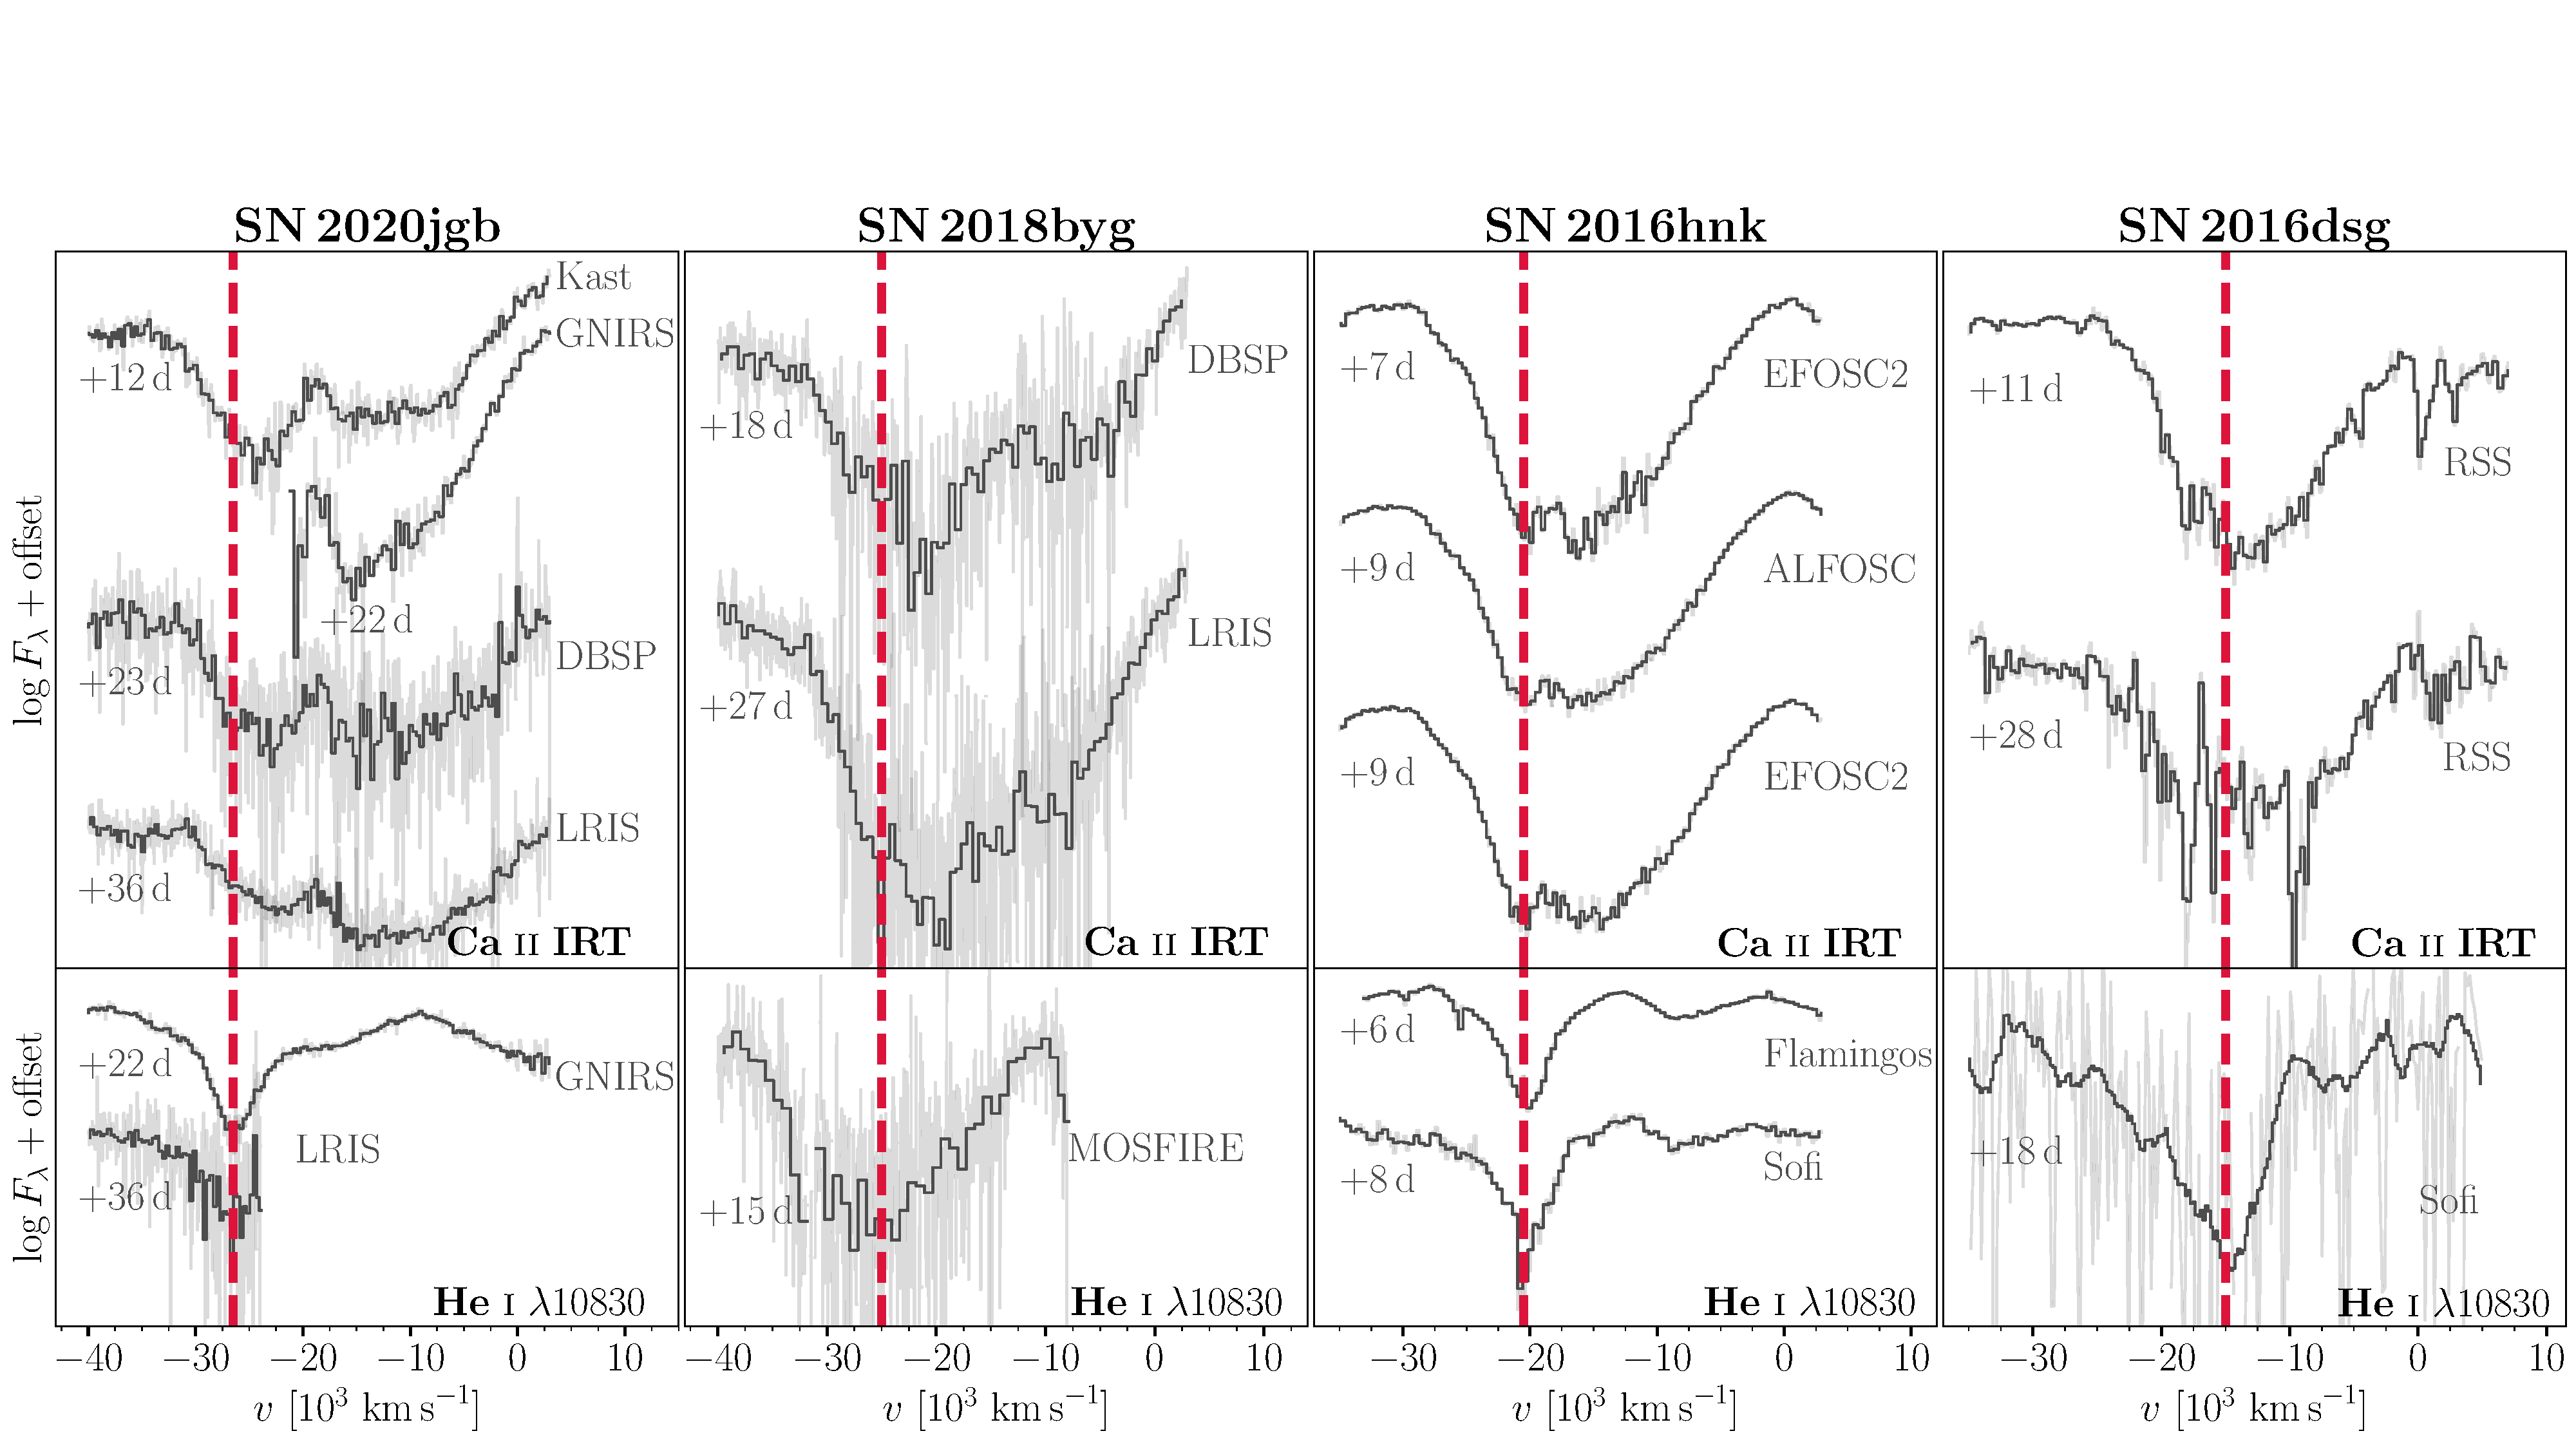
\includegraphics[width=\linewidth]{CaII_HeI_hvf.pdf}
    \label{fig:hvp_comp}
    \caption{Spectra in the velocity space, comparing the high-velocity component of \ion{Ca}{2} IRT and the absorption feature at $\approx$9900 \r{A} assuming it is associated with \ion{He}{1} at 10830 \r{A}.}
\end{figure}

\section{Host Galaxy} \label{sec:host}

\section{Model Comparisons} \label{sec:model}

\section{Discussion and Conclusion} \label{sec:discussion}

\bibliography{SN2020jgb}{}
\bibliographystyle{aasjournal}

%% This command is needed to show the entire author+affiliation list when
%% the collaboration and author truncation commands are used.  It has to
%% go at the end of the manuscript.
%\allauthors

%% Include this line if you are using the \added, \replaced, \deleted
%% commands to see a summary list of all changes at the end of the article.
%\listofchanges

\end{document}

% End of file `sample631.tex'.
